\documentclass[letterpaper,12pt]{article}\usepackage[]{graphicx}\usepackage[]{color}
%% maxwidth is the original width if it is less than linewidth
%% otherwise use linewidth (to make sure the graphics do not exceed the margin)
\makeatletter
\def\maxwidth{ %
  \ifdim\Gin@nat@width>\linewidth
    \linewidth
  \else
    \Gin@nat@width
  \fi
}
\makeatother

\definecolor{fgcolor}{rgb}{0.345, 0.345, 0.345}
\newcommand{\hlnum}[1]{\textcolor[rgb]{0.686,0.059,0.569}{#1}}%
\newcommand{\hlstr}[1]{\textcolor[rgb]{0.192,0.494,0.8}{#1}}%
\newcommand{\hlcom}[1]{\textcolor[rgb]{0.678,0.584,0.686}{\textit{#1}}}%
\newcommand{\hlopt}[1]{\textcolor[rgb]{0,0,0}{#1}}%
\newcommand{\hlstd}[1]{\textcolor[rgb]{0.345,0.345,0.345}{#1}}%
\newcommand{\hlkwa}[1]{\textcolor[rgb]{0.161,0.373,0.58}{\textbf{#1}}}%
\newcommand{\hlkwb}[1]{\textcolor[rgb]{0.69,0.353,0.396}{#1}}%
\newcommand{\hlkwc}[1]{\textcolor[rgb]{0.333,0.667,0.333}{#1}}%
\newcommand{\hlkwd}[1]{\textcolor[rgb]{0.737,0.353,0.396}{\textbf{#1}}}%

\usepackage{framed}
\makeatletter
\newenvironment{kframe}{%
 \def\at@end@of@kframe{}%
 \ifinner\ifhmode%
  \def\at@end@of@kframe{\end{minipage}}%
  \begin{minipage}{\columnwidth}%
 \fi\fi%
 \def\FrameCommand##1{\hskip\@totalleftmargin \hskip-\fboxsep
 \colorbox{shadecolor}{##1}\hskip-\fboxsep
     % There is no \\@totalrightmargin, so:
     \hskip-\linewidth \hskip-\@totalleftmargin \hskip\columnwidth}%
 \MakeFramed {\advance\hsize-\width
   \@totalleftmargin\z@ \linewidth\hsize
   \@setminipage}}%
 {\par\unskip\endMakeFramed%
 \at@end@of@kframe}
\makeatother

\definecolor{shadecolor}{rgb}{.97, .97, .97}
\definecolor{messagecolor}{rgb}{0, 0, 0}
\definecolor{warningcolor}{rgb}{1, 0, 1}
\definecolor{errorcolor}{rgb}{1, 0, 0}
\newenvironment{knitrout}{}{} % an empty environment to be redefined in TeX

\usepackage{alltt}
\usepackage[top=1in,bottom=1in,left=1in,right=1in]{geometry}
\usepackage{setspace}
\usepackage[colorlinks=true,urlcolor=blue,citecolor=blue,linkcolor=blue]{hyperref}
\usepackage{indentfirst}
\usepackage{multirow}
\usepackage{booktabs}
\usepackage[final]{animate}
\usepackage{graphicx}
\usepackage{verbatim}
\usepackage{rotating}
\usepackage{tabularx}
\usepackage{array}
\usepackage{subfig} 
\usepackage[noae]{Sweave}
\usepackage{cleveref}
\usepackage[figureposition=bottom]{caption}
\usepackage{paralist}
\usepackage{acronym}
\usepackage{outlines}
\usepackage{pdflscape}

% knitr options




\IfFileExists{upquote.sty}{\usepackage{upquote}}{}
\begin{document}

\begin{landscape}
\centering\vspace*{\fill}
\begin{figure}[!ht]

{\centering 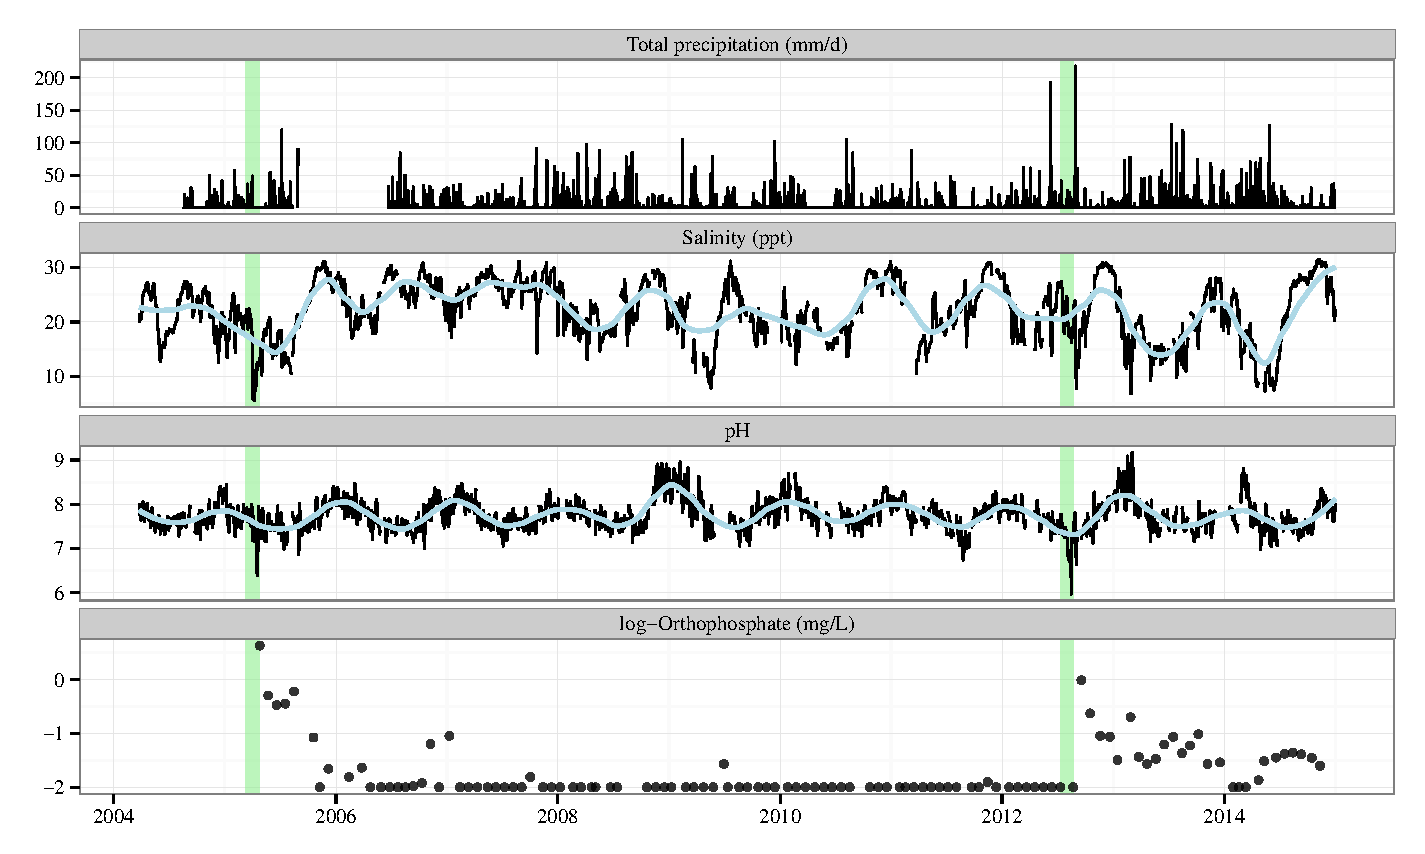
\includegraphics[width=\maxwidth]{figs/tsplot-1} 

}

\caption[Time series of total precipitation, salinity, pH, and phosphate for Bangs Lake, Grand Bay reserve]{Time series of total precipitation, salinity, pH, and phosphate for Bangs Lake, Grand Bay reserve.  Vertical green bars indicate a heavy rain event in April 2005 and hurricane Isaac in August 2012.  Salinity and pH include a loess smooth to reduce variability.}\label{fig:tsplot}
\end{figure}


\end{landscape}
\clearpage

\begin{figure}[!ht]

{\centering 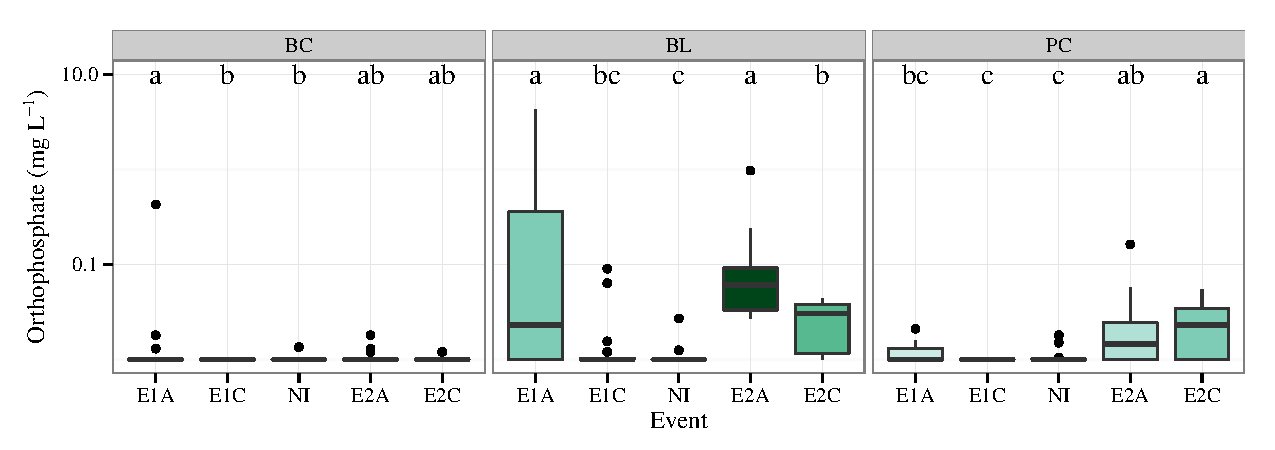
\includegraphics[width=\maxwidth]{figs/tukey-1} 

}

\caption[Boxplot summaries of nutrient data at Bangs Lake, Grand Bay grouped by events]{Boxplot summaries of nutrient data at Bangs Lake, Grand Bay grouped by events.  Letters indicate events for each nutrient with significantly different observations based on Tukey multiple comparison analysis.  Boxes represent the interquartile range (IQR, 25\textsuperscript{th} to 75\textsuperscript{th} percentile) with the median as the middle horizonal line.  Outliers are present beyond whiskers (1.5$\cdot$IQR). E1A: event 1 acute, E1C: event 1 chronic, NI: non-impact, E2A: event 2 acute, E2C: event 2 chronic.}\label{fig:tukey}
\end{figure}


\clearpage

\begin{figure}[!ht]

{\centering 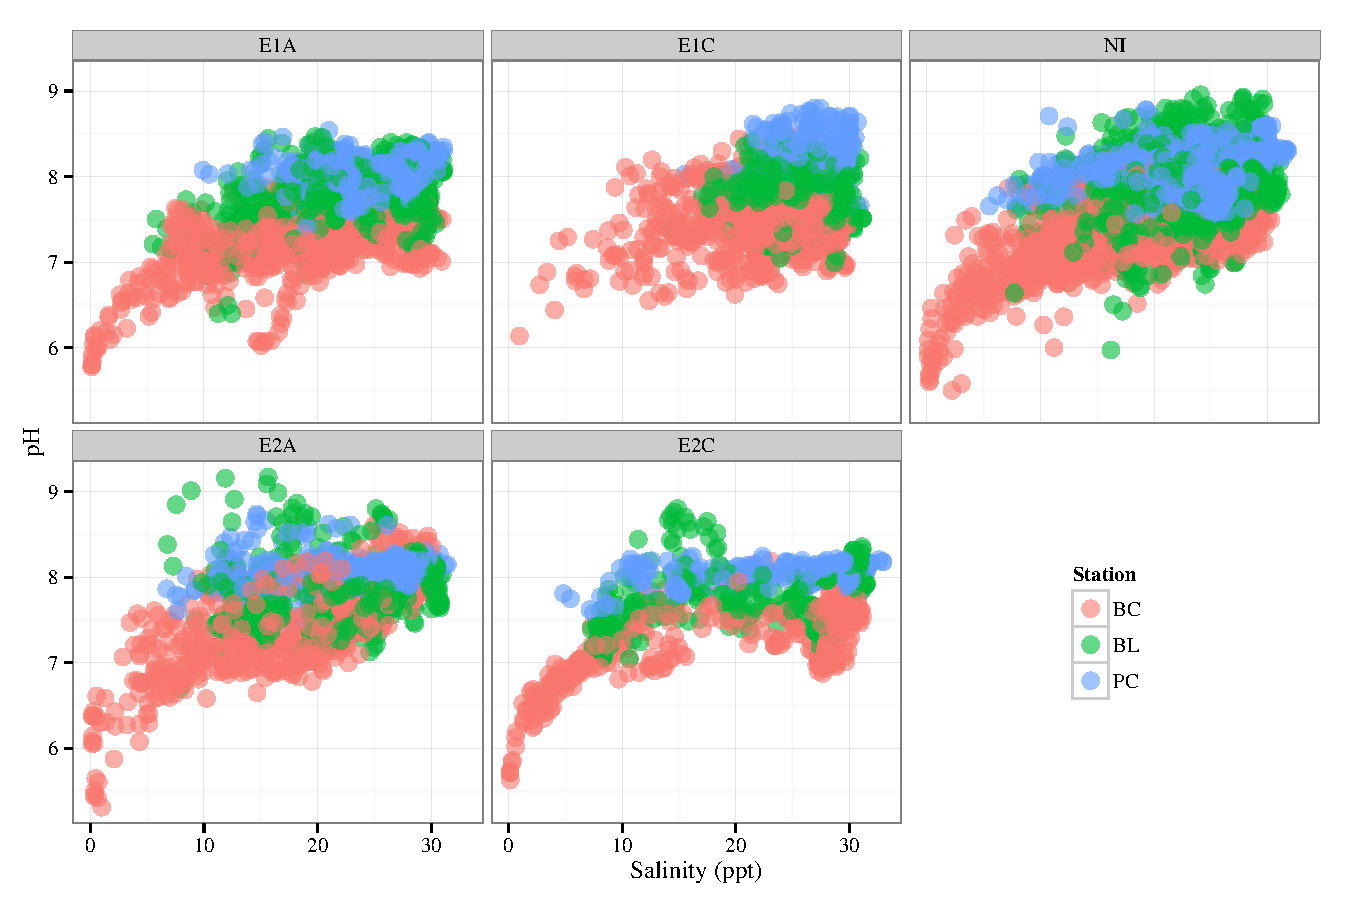
\includegraphics[width=\maxwidth]{figs/phvsal1-1} 

}

\caption[Scatterplots of pH versus salinity for each of the time frames, grouped by station]{Scatterplots of pH versus salinity for each of the time frames, grouped by station.  Observations are daily averages from the continuous time series. E1A: event 1 acute, E1C: event 1 chronic, NI: non-impact, E2A: event 2 acute, E2C: event 2 chronic.}\label{fig:phvsal1}
\end{figure}


\clearpage

\begin{figure}[!ht]

{\centering 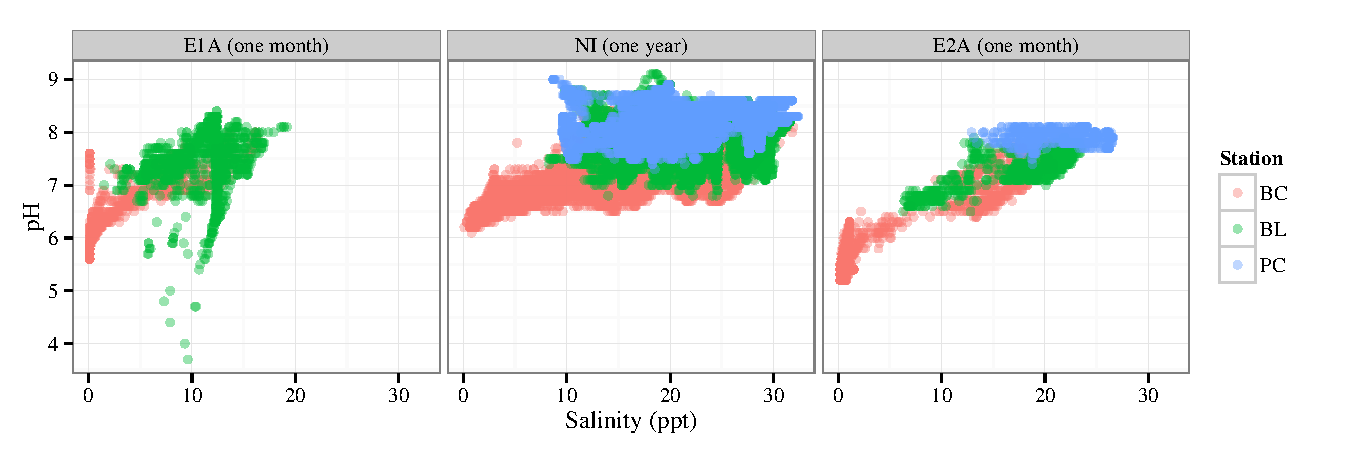
\includegraphics[width=\maxwidth]{figs/phvsal2-1} 

}

\caption[Scatterplots of pH versus salinity for one month following the two acute exposure events (E1A, E2A) and 2010 during the non-impact (NI) time frame]{Scatterplots of pH versus salinity for one month following the two acute exposure events (E1A, E2A) and 2010 during the non-impact (NI) time frame.  Values are thirty-minute observations at each station. E1A: event 1 acute, NI: non-impact, E2A: event 2 acute.}\label{fig:phvsal2}
\end{figure}


\clearpage


\clearpage

\end{document}
